\section{CI Pipeline/Workflow}
\subsection{Overview}
\paragraph{What is a Azure Pipeline/ Github Action?}
Both are the platform for \gls{CI/CD}.

\paragraph{What is a pipeline/ workflow?}
%TODO: CI
A worflow or a pipeline is the configured process that runs the job an a virtual machine (runner/agents) using a runner/ agent.

\paragraph{What is a runner/ agent?}
A runner or agent has two means
\begin{itemize}
	\item the computing infrastructures like a VM or a container
	\item the software installed on the VM to execute the workflow/ pipeline.
\end{itemize}

With regards to \textit{Azure pipelines}, \href{https://learn.microsoft.com/en-us/dotnet/architecture/devops-for-aspnet-developers/actions-vs-pipelines}{Agents}. Azure Pipeline runs on agents. The agent is written in .Net an can run on windows, linus and macOs. 

\paragraph{Keyword Matching}
The two platforms use similar concepts, but with different names.

\begin{figure}[H]
	\centering
	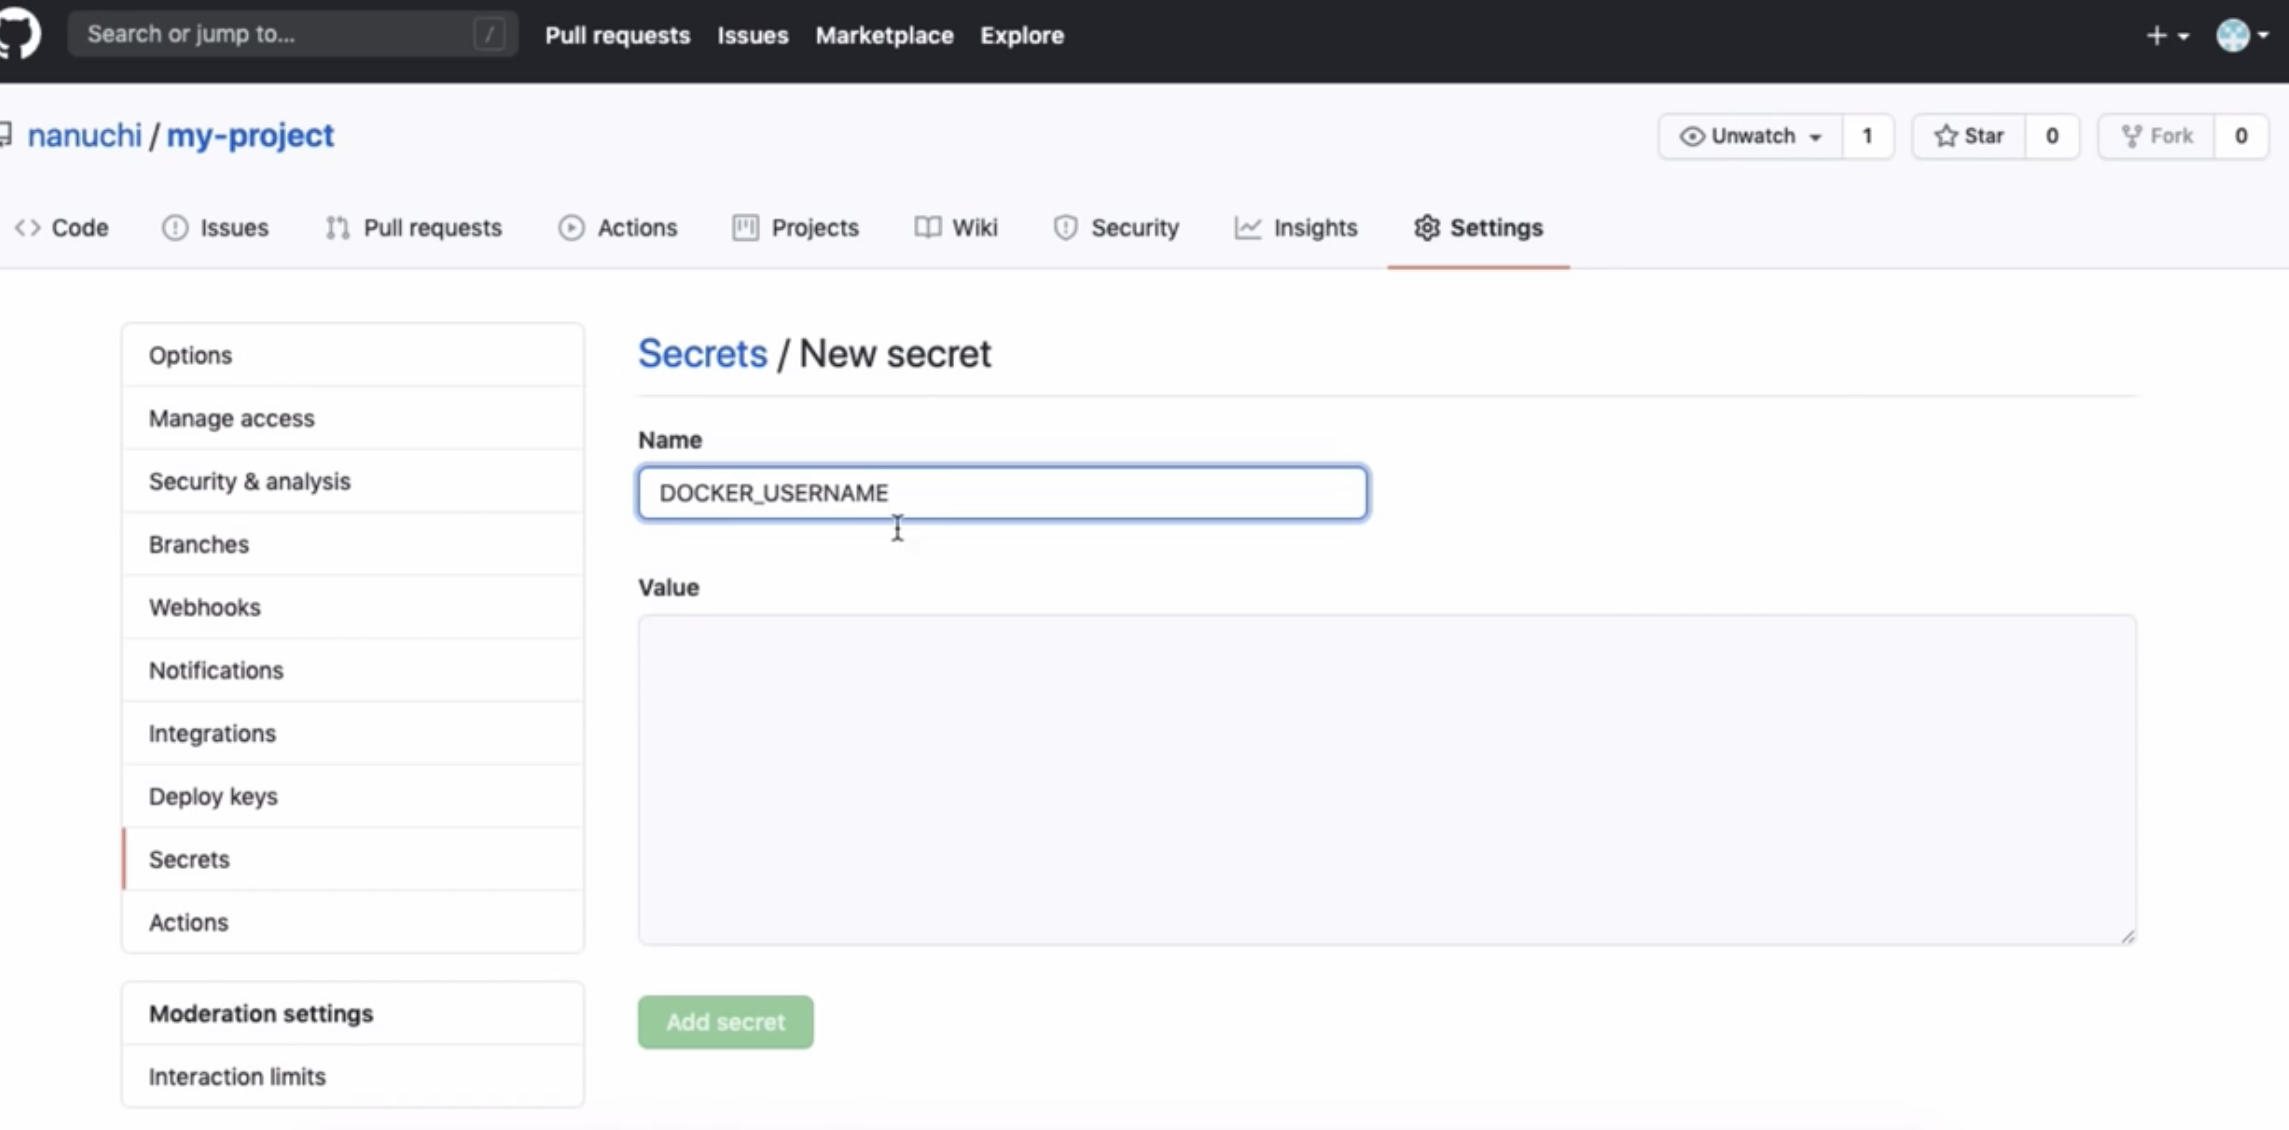
\includegraphics[scale = 0.2]{attachment/chapter_2/Scc106}
	\caption{Keyword matching}
\end{figure}

\begin{itemize}
	\item Scirpt is a script
	\item In Azure a task and in GitHub a Action is reusable code to automate the scipt part.
\end{itemize}


\subsection{GitHub Workflow}
\subsubsection{Aufbau}
Github bietet \textit{Github Actions} an. Dies haben das Ziel \textit{Workflows} zu automatisieren. 

\begin{figure}[H]
	\centering
	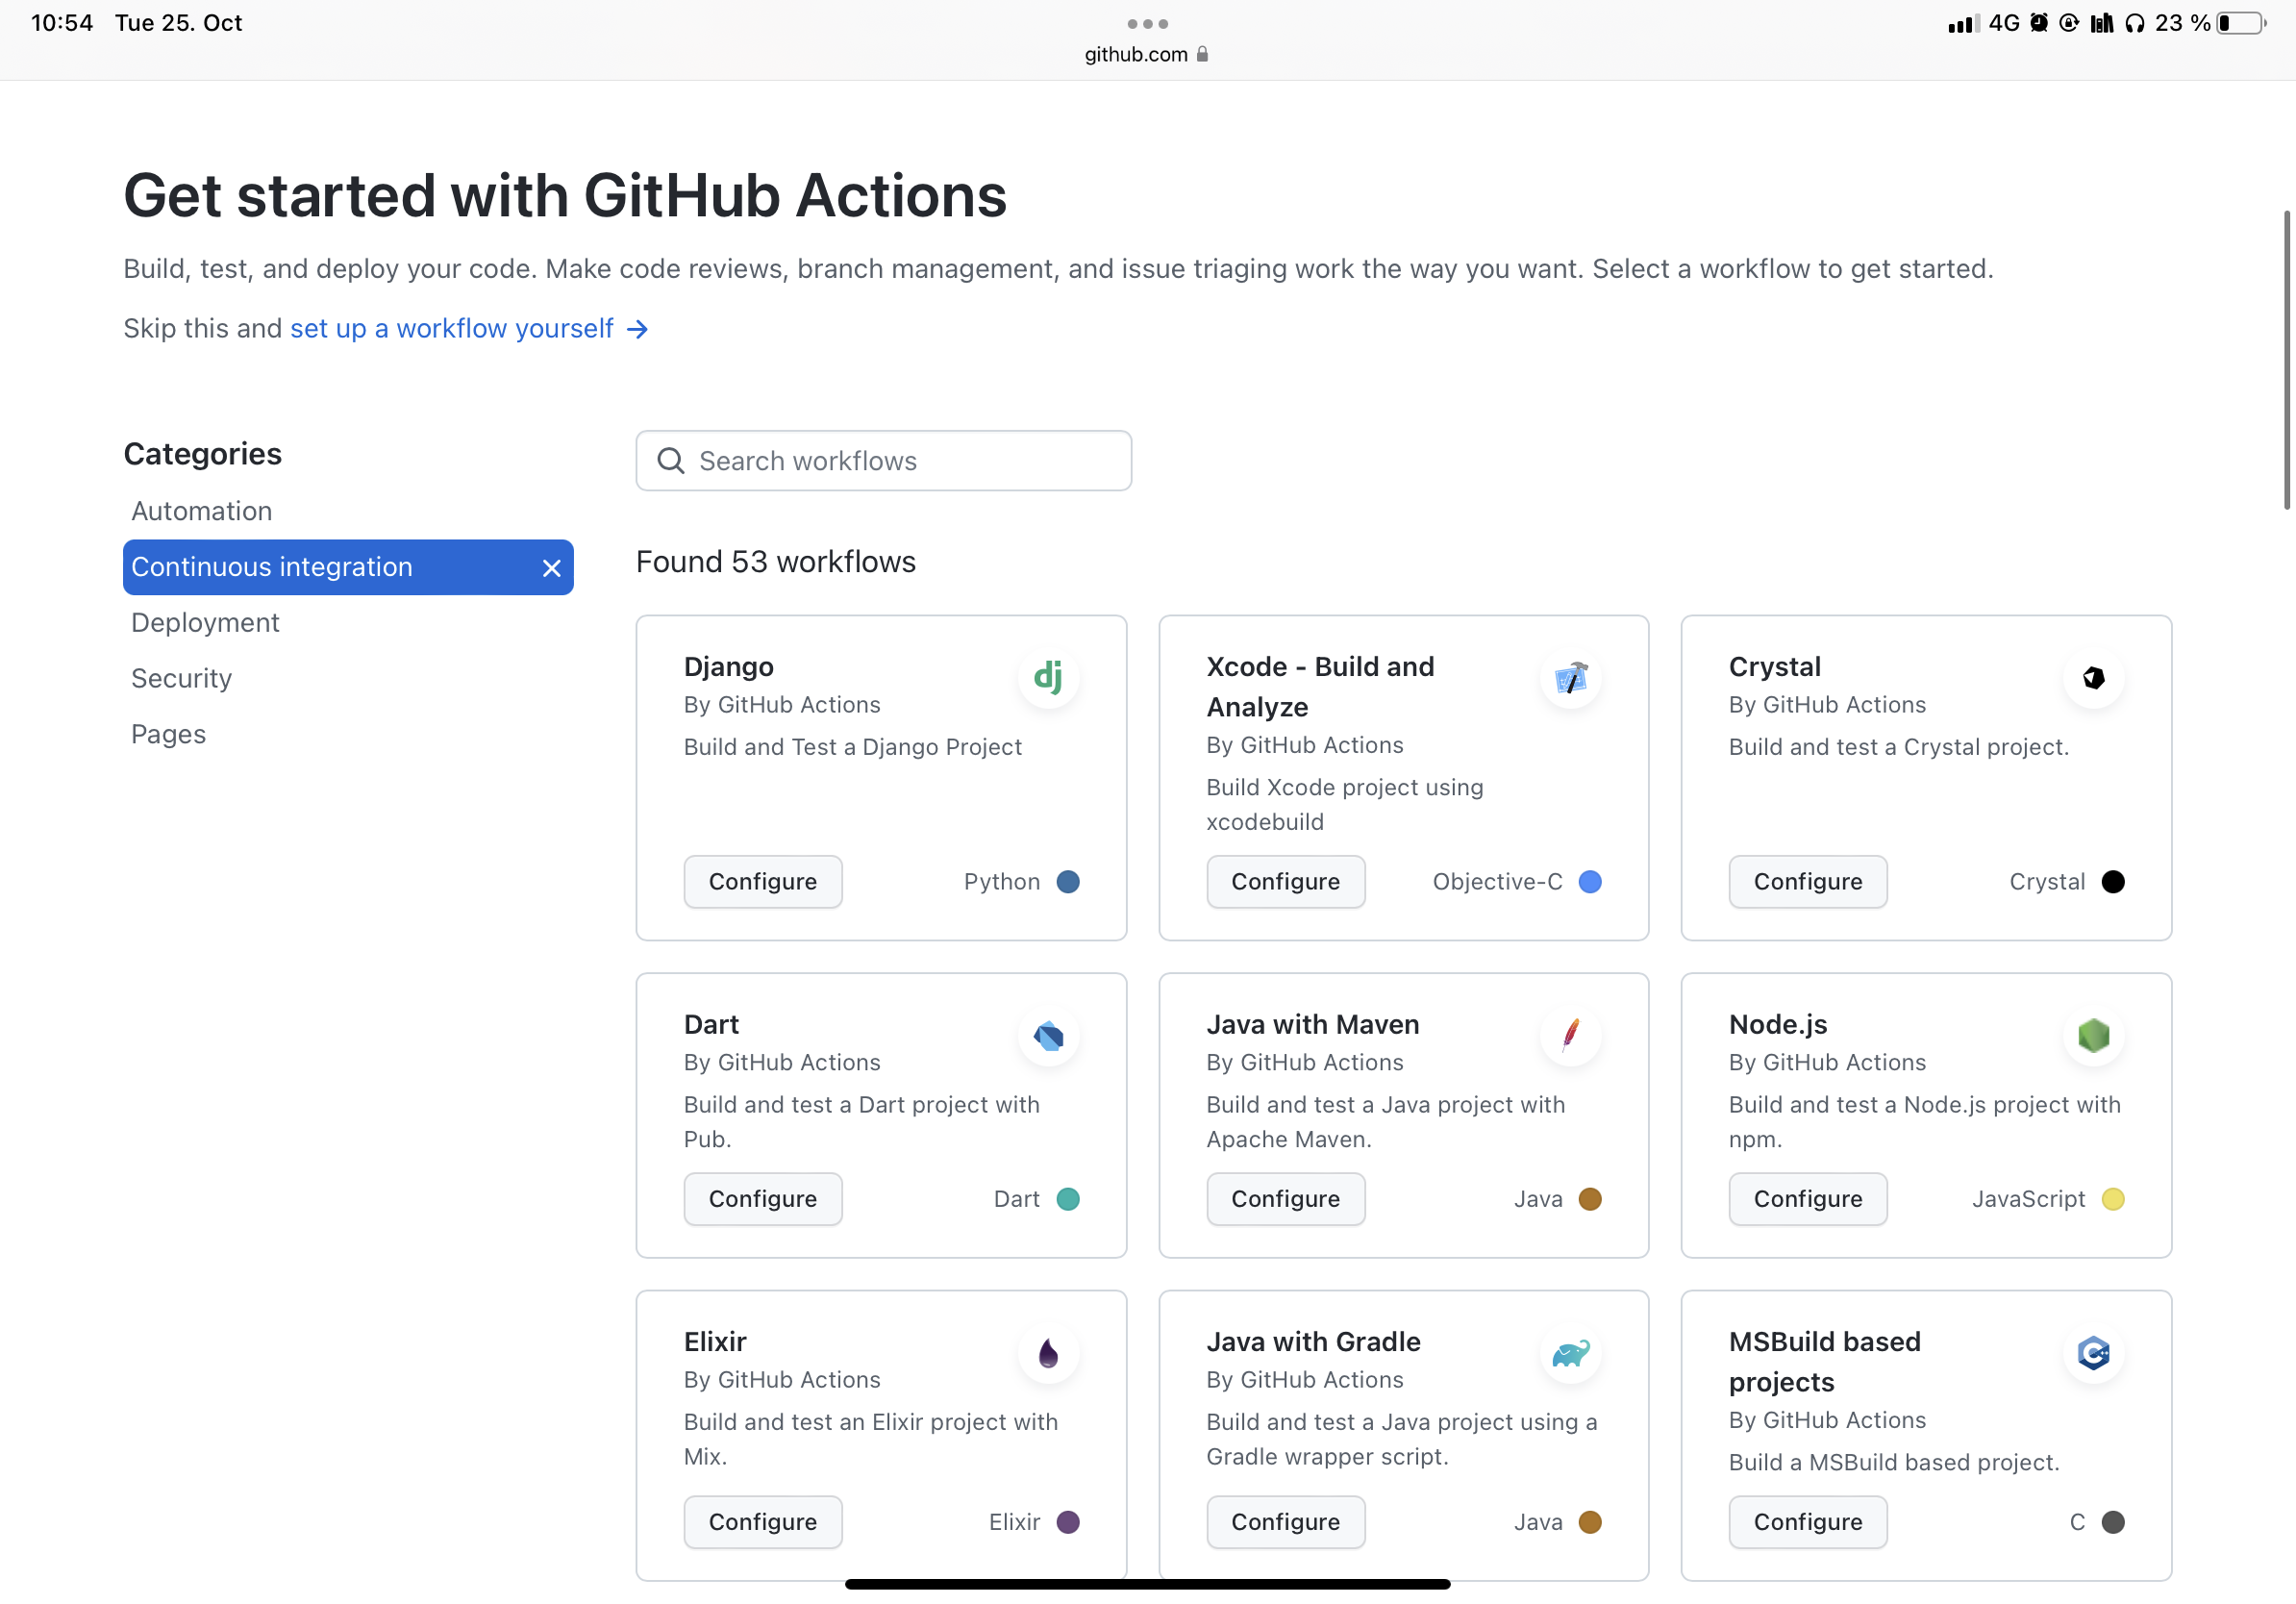
\includegraphics[scale = 0.2]{attachment/chapter_2/Scc098}
	\caption{Reiter Ansicht $"$Action$"$/ Continuous Integration}
\end{figure}

Dabei handelt es sich nicht außschließlich um CI/CD Prozesse. Ebenso können beispielweise Label-Zuweisungen durchgeführt werden.


\begin{figure}[H]
	\centering
	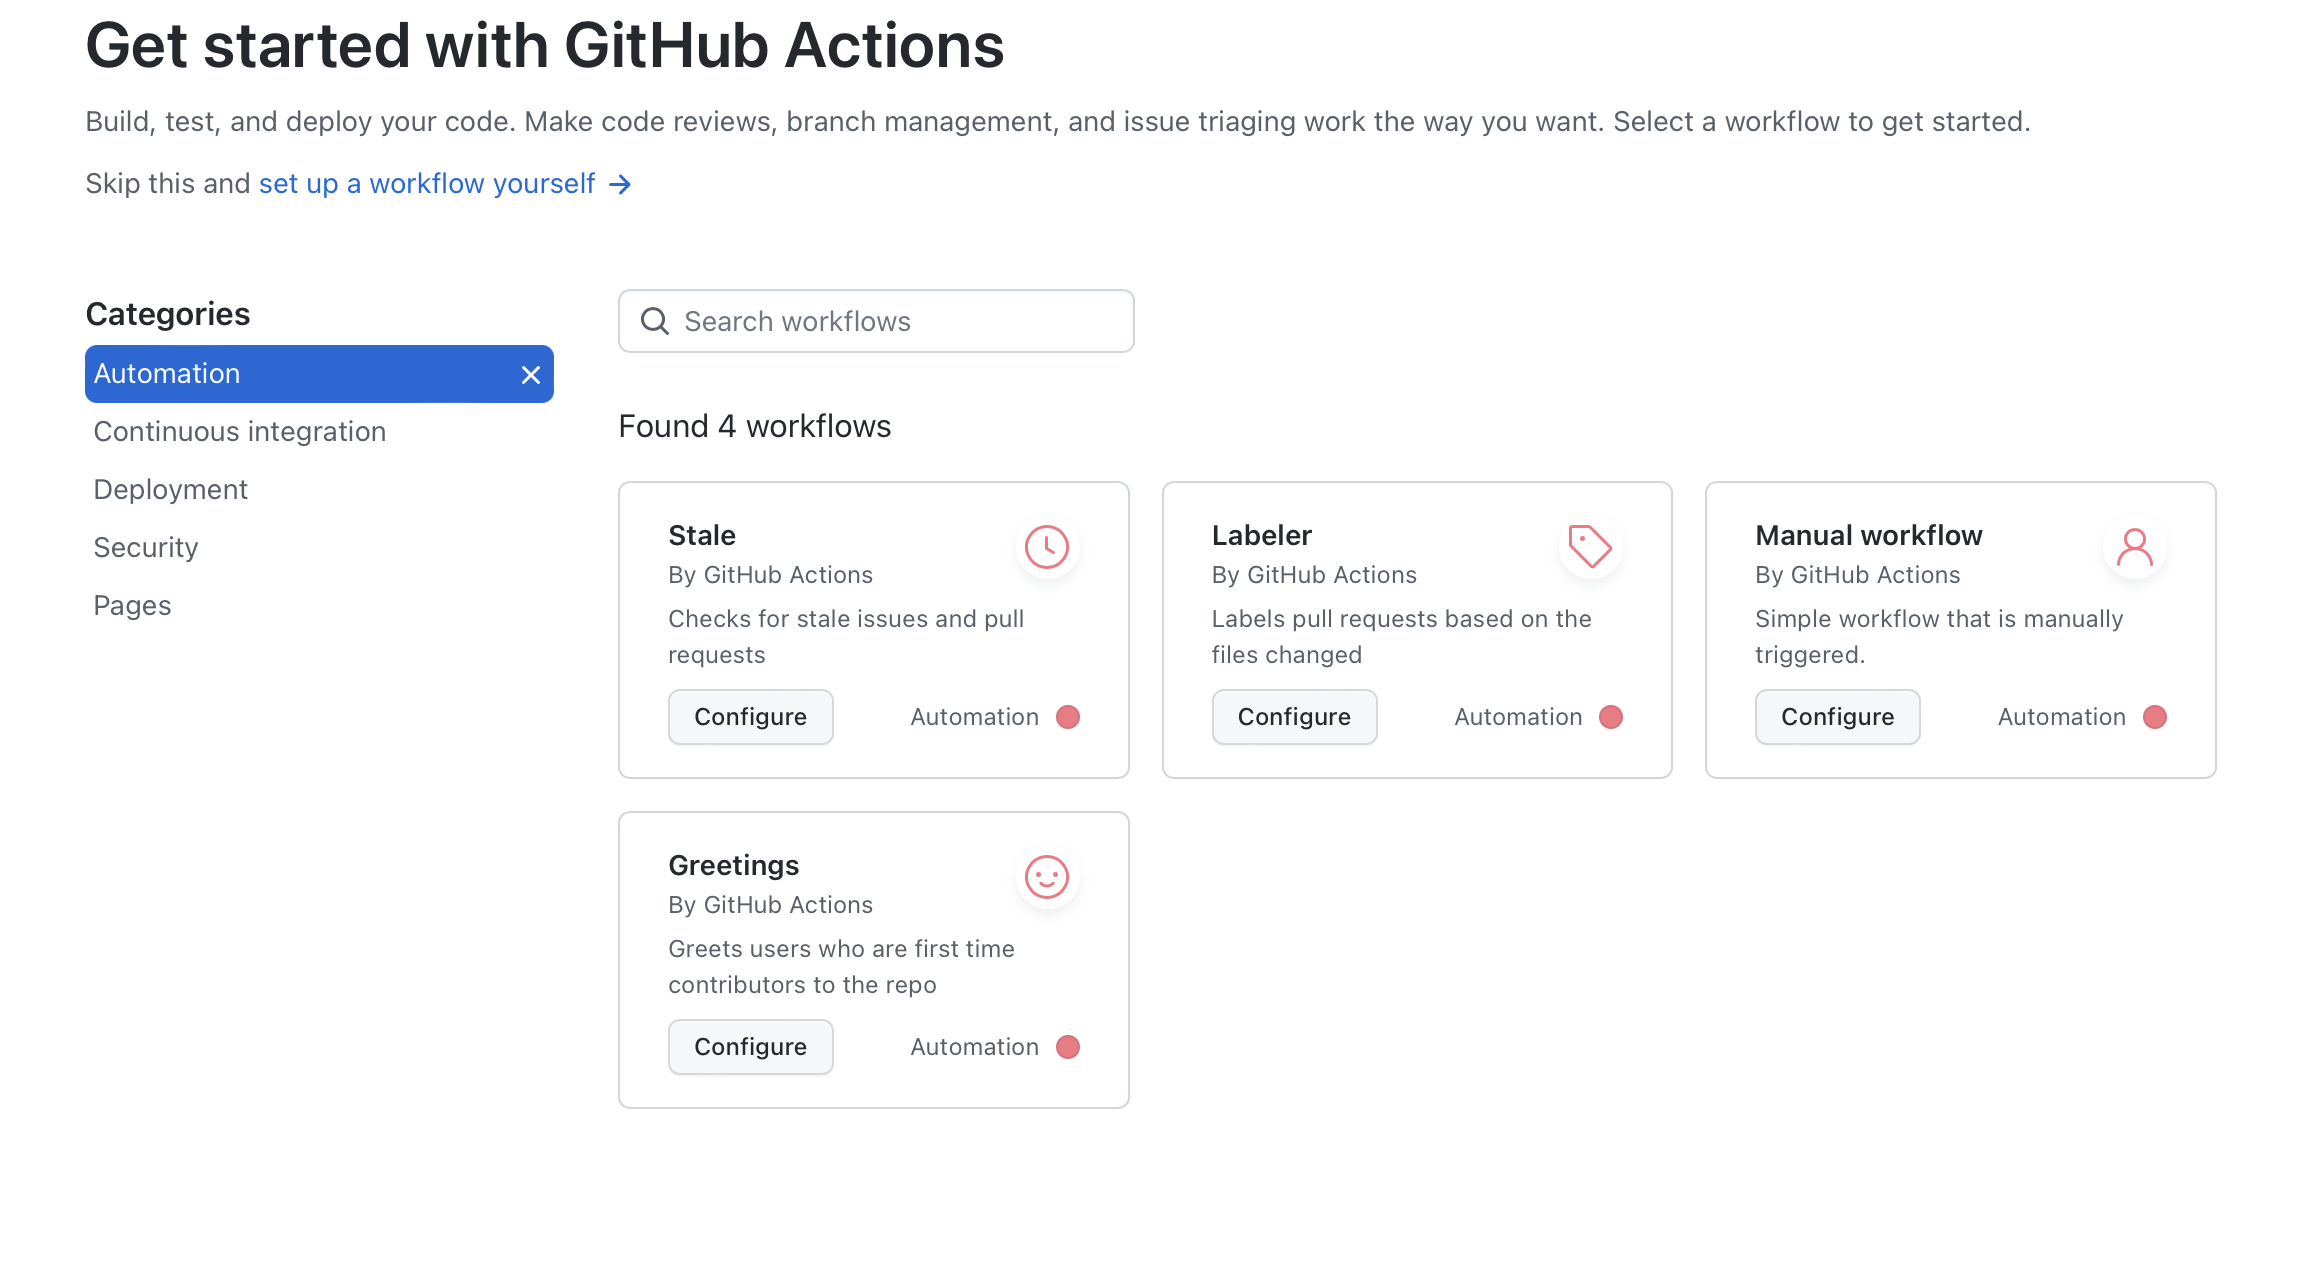
\includegraphics[scale = 0.2]{attachment/chapter_2/Scc099}
	\caption{Reiter Ansicht $"$Action$"$/ Automation}
\end{figure}

Ein Workflow setzt sich aus
\begin{itemize}
	\item Events, welches den Workflow (Github Action) auslösen und
	\item den Jobs, welche die automatisierten Schritte enthalten.
\end{itemize}
Ein Job besteht aus einem oder mehreren Schritten. Ein Schritt kann eine \textit{GitHub Action} - \textbf{uses} oder ein Kommando - \textbf{run} sein.

\begin{figure}[H]
	\centering
	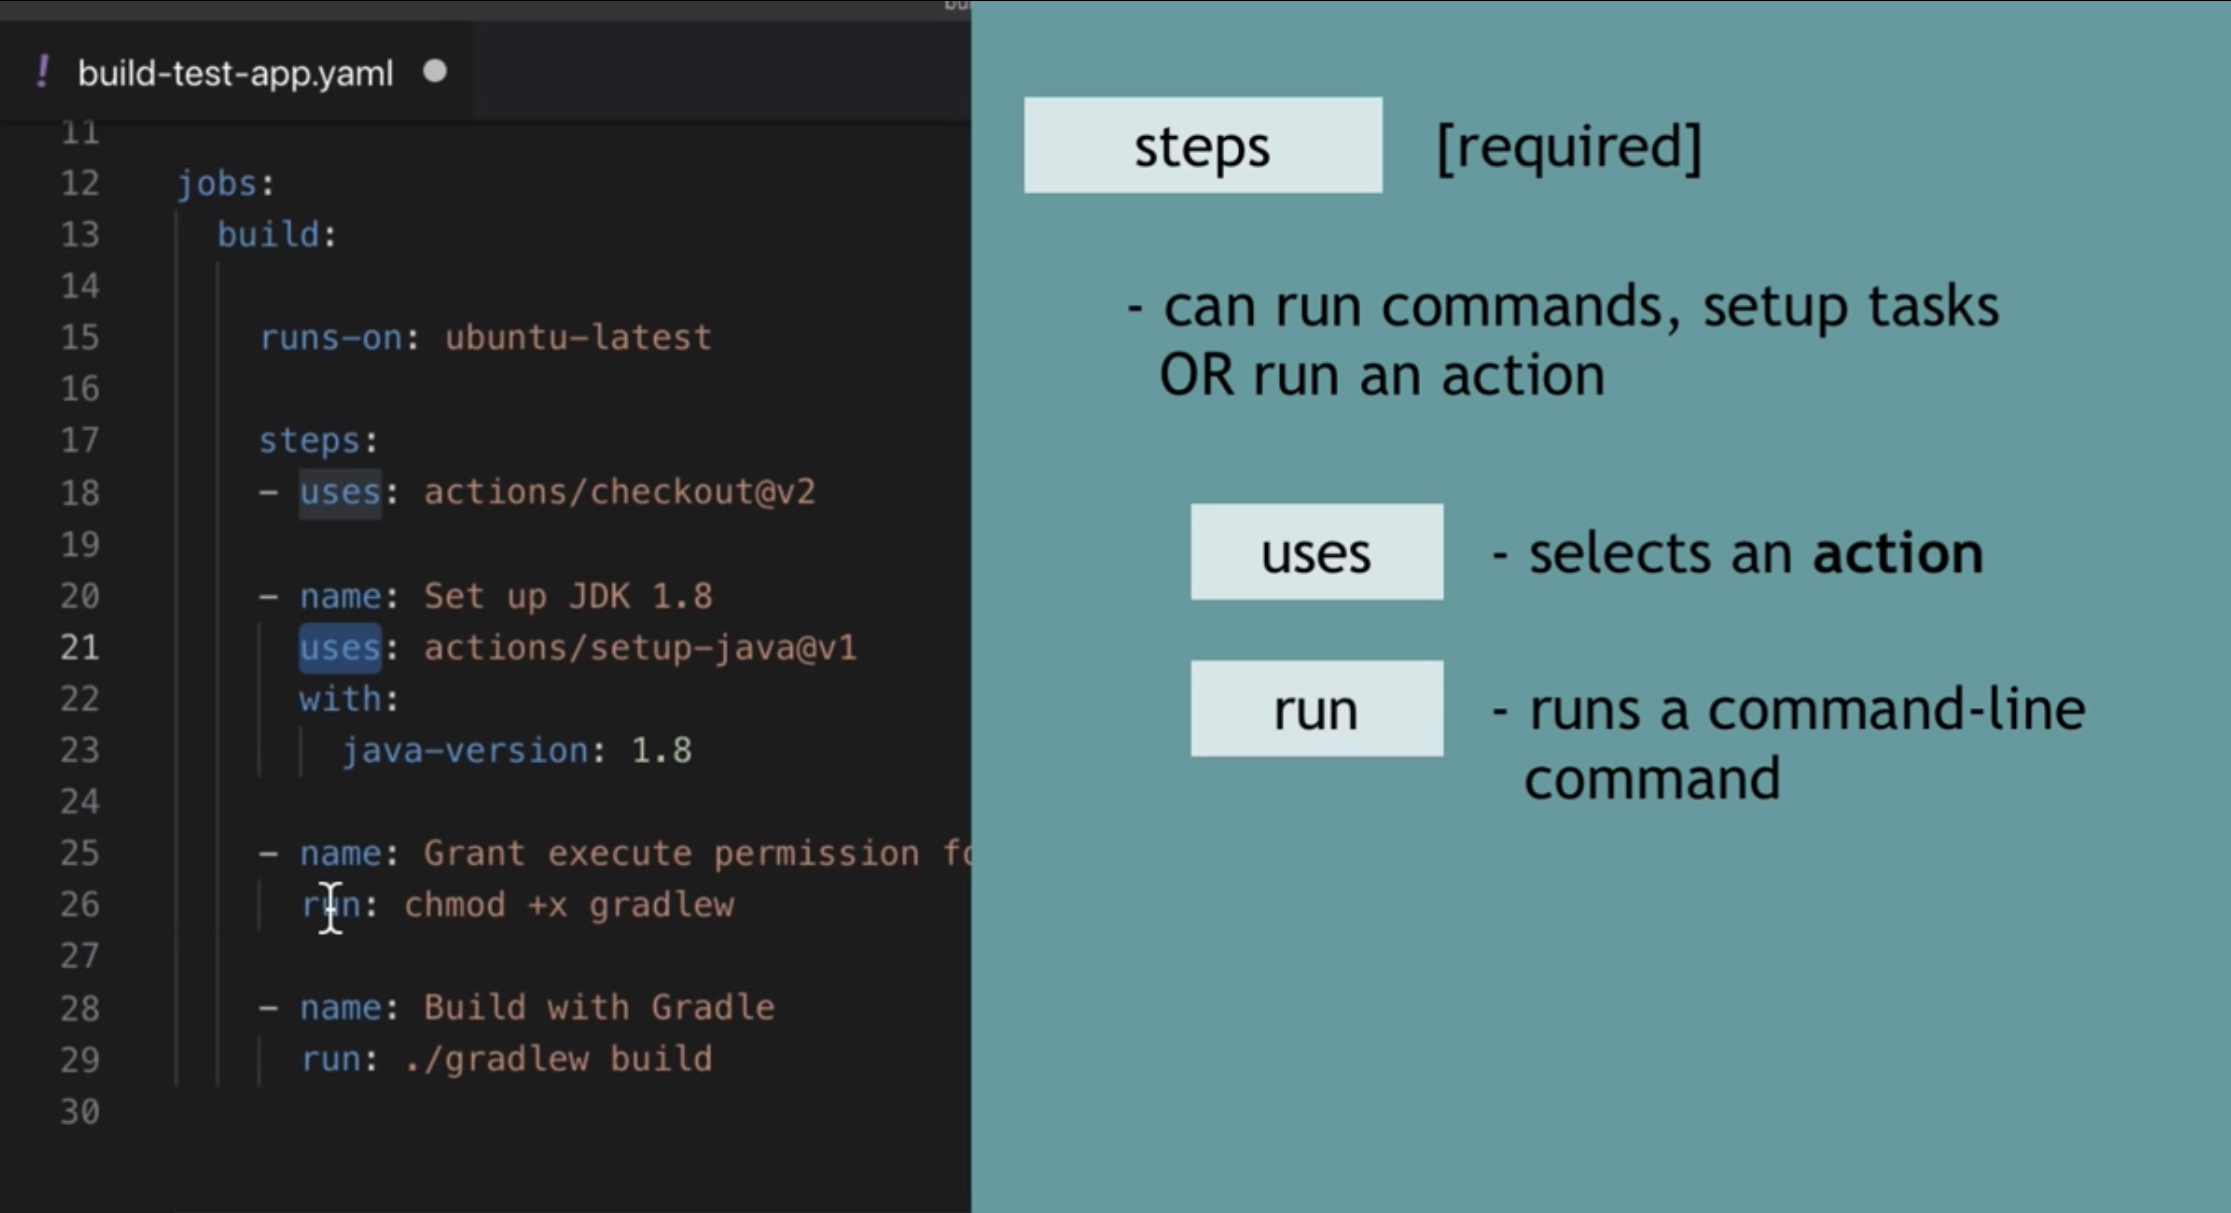
\includegraphics[scale = 0.2]{attachment/chapter_2/Scc100}
	\caption{Aufbau eines Job}
\end{figure}

Jeder Schritt kann mit einem Namen (\textit{name:}) versehen werden. Dieser wird bei der Ausführung des Schrittes verwendet, wenn um eine bessere Beschreibung zu ermöglichen.

Der Job wird mit ebenso mit einem eigenen Namen versehen. Im angeführten Beispiel, ist es \textit{build}. Jeder Job wird ein einer \textit{runner environment} ausgeführt. Diese muss spezifisch angegeben werden. Es werden drei Betriebssysteme unterstützt: Ubuntu (Linux), Windows, macOS. Der Default-Wert für die Version ist \textit{-latest}.

\begin{lstlisting}[style=Config, caption={GitHub Runner}, captionpos=b]
	...
	runs-on: ubuntu-latest, windows-latest, macOC-latest
	...
\end{lstlisting}

GitHub unterstütz nur spezifische Betriebssystem Angaben.\footnote{
	Wenn andere Versionen benötigt werden, ist dies under der Dokumentation für GitHub Aktion zu finden.
}	

Jeder Job wird in einer neuen \gls{VEN} - \textbf{GitHub Action Runner} ausgeführt.

\begin{figure}[H]
	\centering
	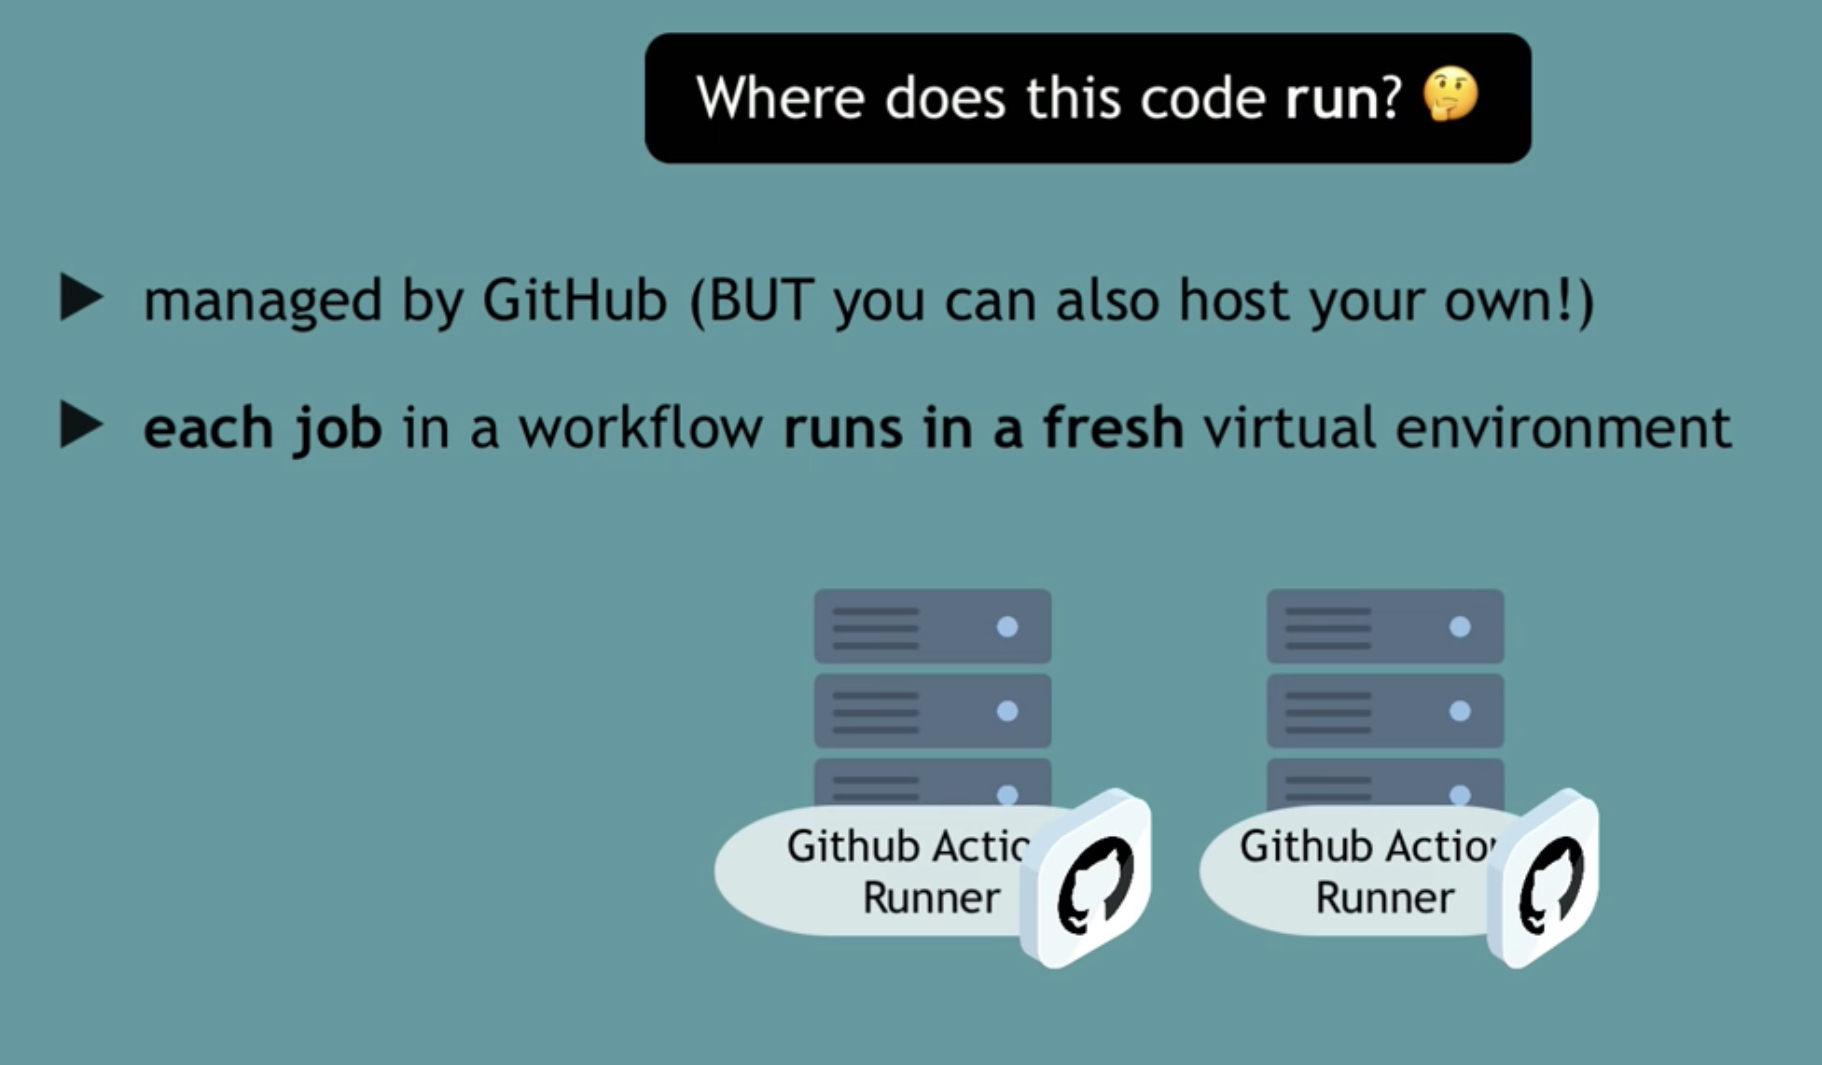
\includegraphics[scale = 0.2]{attachment/chapter_2/Scc101}
	\caption{Github Action Runner}
\end{figure}


Gespeichert wird eine GitHub Action unter \textit{.github/workflow/}

\begin{figure}[H]
	\centering
	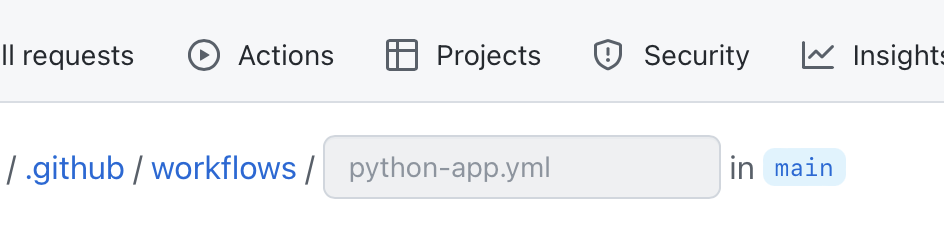
\includegraphics[scale = 0.2]{attachment/chapter_2/Scc104}
	\caption{Speicherort}
\end{figure}

\paragraph{(GitHub) Actions}

Wie schon erwähnt, kann ein Schritt ein vordefinierte Action ausgeführt werden (\textit{uses}) oder ein Kommando (\textit{run}). Am Beispiel von \textit{checkout} wird gezeigt, was sich hinter einem Aktion verbirgt.
\begin{lstlisting}[style=Config, caption={GitHub Action: Checkout}, captionpos=b]
	...
	steps:
	- uses: actions/checkout@v2 // find the commited oder merge (pull) point.
	...
\end{lstlisting}
Der Verzeichnis \textit{actions} verweist auf github.com/actions. Dort finden sich alle verfügbaren Repositories. Jede Action ist ein eigenes Repository, welches die automatisierten Schritt beinhaltet. Jedes Repo kann untersucht werden, was genau dort getan wird. Under \textit{actions/checkout} ist unter \textit{action.yml} der genaue Vorgang zu finden. Diese spezielle Aktion finden den SHA Punkt für das Event, welchen den Workflow ausgelöst hat. Dies könnte ein Commit oder pull-request (Merge-Request) sein.

\begin{figure}[H]
	\centering
	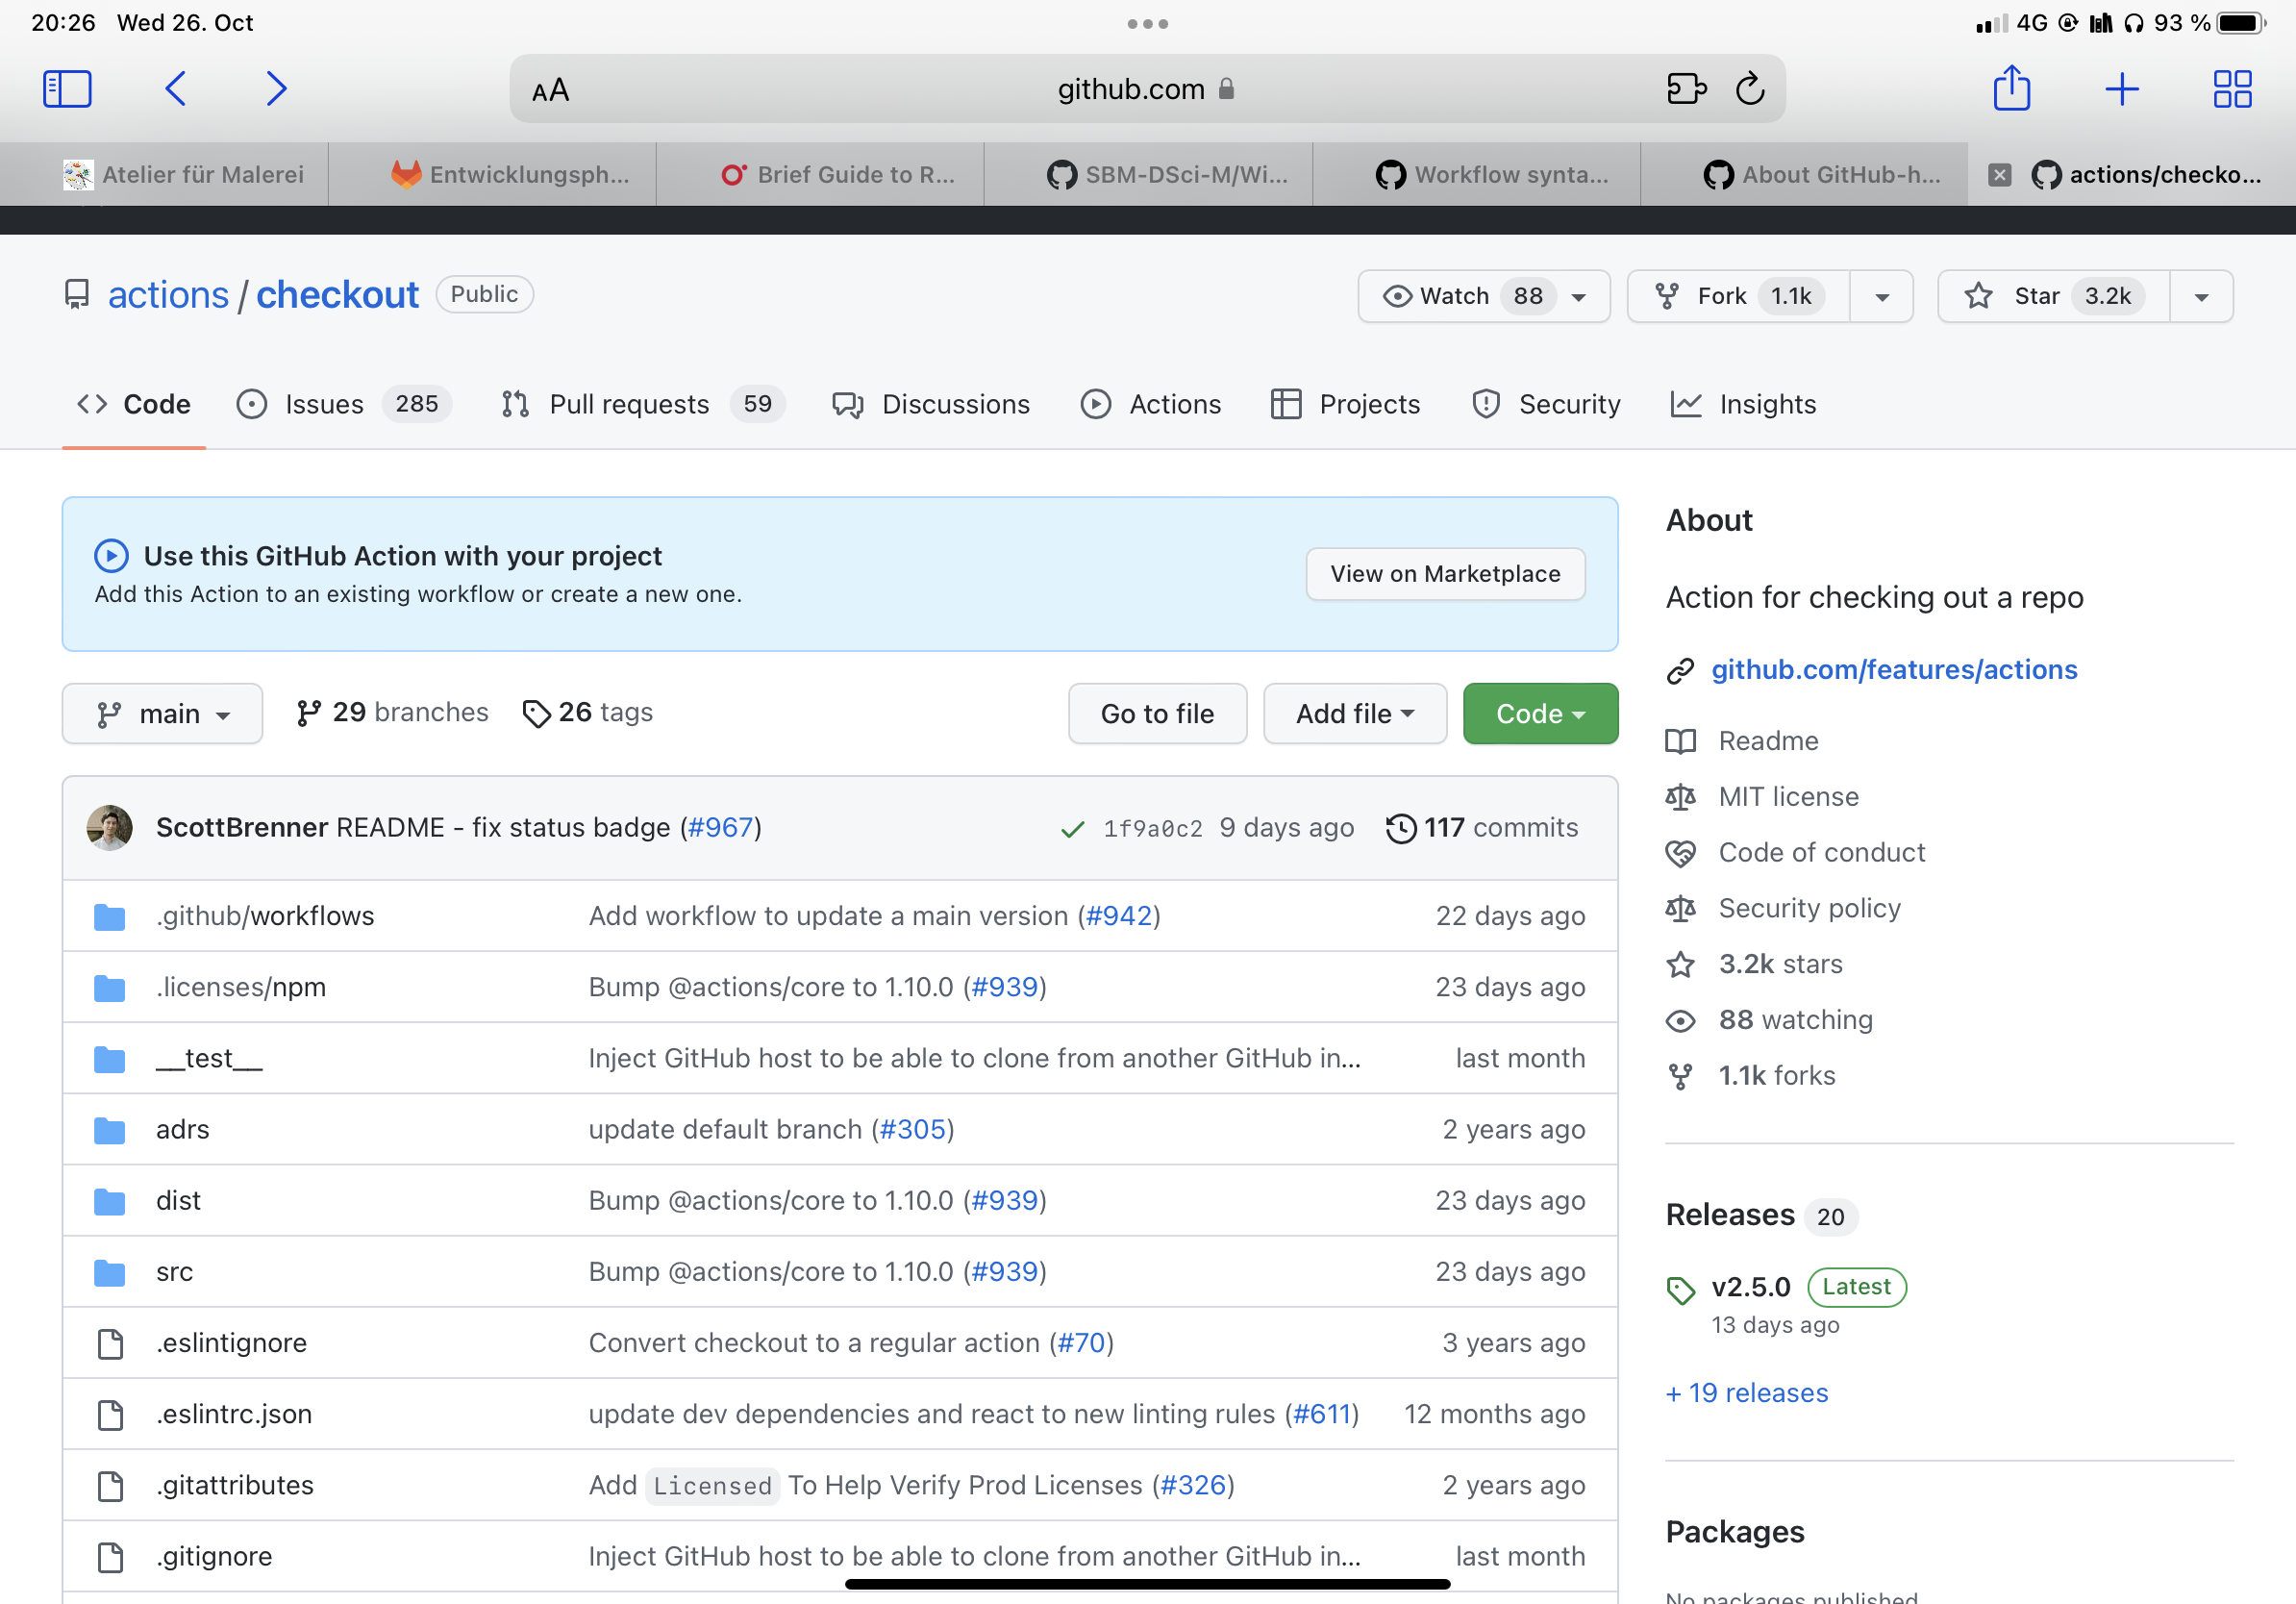
\includegraphics[scale = 0.2]{attachment/chapter_2/Scc102}
	\caption{Github Action/checkout}
\end{figure}

Wie bei anderen Repos wird auch bei diesen eine Versionnummer $"$@v2$"$ mit gegeben. Unter \textit{actions} sind die über GitHub vertriebenen.

\begin{lstlisting}[style=Config, caption={Extern Action}, captionpos=b]
	...
	steps:
	- uses: mr-smiths-exellent/docker-build-push@v4
	...
\end{lstlisting}

\paragraph{Matrix Strategy}
Ein \textit{matrix stategy} lässt verschiedene variablen in Kombination zu einander in einem Job (Teil des Workflows) aufführen lassen. Dies erlaubt bis zu 256 Jobs in eine Job ausführen zu lassen. Die Matrix wird mit verschiedenen Variablen befüllt. Dies können in der Combination über \textit{matrix.<>} angesteuert werden. Um die Matrix zu definieren, wird \textit{jobs.<job-id>.strategy.matrix} benötigt.

\begin{lstlisting}[style=Config, caption={GitHub matrix strategy}, captionpos=b]
	jobs: 				//jobs
	test_job_name:	//jobs.job_id
	strategy:		//jobs.job_id.strategie
	matrix:	//jobs.job_id.strategie.matrix
	version: [10,12,14] // jobs.job_id.strategie.matrix.version
	os: [ubuntu-latest, windows-latest] // jobs.job_id.strategie.matrix.os
\end{lstlisting}
Wir der Job \textit{test-job-name} ausgeführt, so wird
\begin{itemize}
	\item $\left\lbrace \right.$ version: 10, os: ubuntu-latest $\left. \right\rbrace$
	\item $\left\lbrace \right.$ version: 12, os: ubuntu-latest $\left. \right\rbrace$
	\item $\left\lbrace \right.$ version: 14, os: ubuntu-latest $\left. \right\rbrace$
	\item $\left\lbrace \right.$ version: 10, os: windows-latest $\left. \right\rbrace$
	\item $\left\lbrace \right.$ version: 12, os: windows-latest $\left. \right\rbrace$
	\item $\left\lbrace \right.$ version: 14, os: windows-latest $\left. \right\rbrace$
\end{itemize}
Job Konfiguration ausgeführt. \\

In dem Job können die Kombinationen mit $\left\lbrace \left\lbrace matrix.<> \right\rbrace\right\rbrace$ erreicht werden.

\begin{lstlisting}[style=Config, caption={Single Dimension Matrix}, captionpos=b]
	jobs:
	example_matrix:
	strategy:
	matrix:
	version: [10, 12, 14]
	steps:
	- uses: actions/setup-node@v3
	with:
	node-version: ${{ matrix.version }}
\end{lstlisting}

\begin{lstlisting}[style=Config, caption={Multi Dimension Matrix}, captionpos=b]
	jobs:
	example_matrix:
	strategy:
	matrix:
	os: [ubuntu-22.04, ubuntu-20.04]
	version: [10, 12, 14]
	runs-on: ${{ matrix.os }}
	steps:
	- uses: actions/setup-node@v3
	with:
	node-version: ${{ matrix.version }}
\end{lstlisting}
Vermerk: Es scheint, die Strategy muss nicht am Anfang definiert werden. 

$\$ \left\lbrace \left\lbrace matrix.os\right\rbrace\right\rbrace$ ist auf vor der Defininierung der Strategie erreichbar.


\begin{lstlisting}[style=Config, caption={Multi Dimension Matrix}, captionpos=b]
	jobs:
	example_matrix:
	runs-on: ${{ matrix.os }}
	strategy:
	matrix:
	os: [ubuntu-22.04, ubuntu-20.04]
	version: [10, 12, 14]
	steps:
	- uses: actions/setup-node@v3
	with:
	node-version: ${{ matrix.version }}
\end{lstlisting}
%TODO: Test
% Kontrolle, ob die Reihenfolge eingehalten wird.


\subsubsection{Python Packete Testing}
Wie oben gezeigt, bietet Github Action Vorlagen für Autommatisierungen an.

\begin{figure}[H]
	\centering
	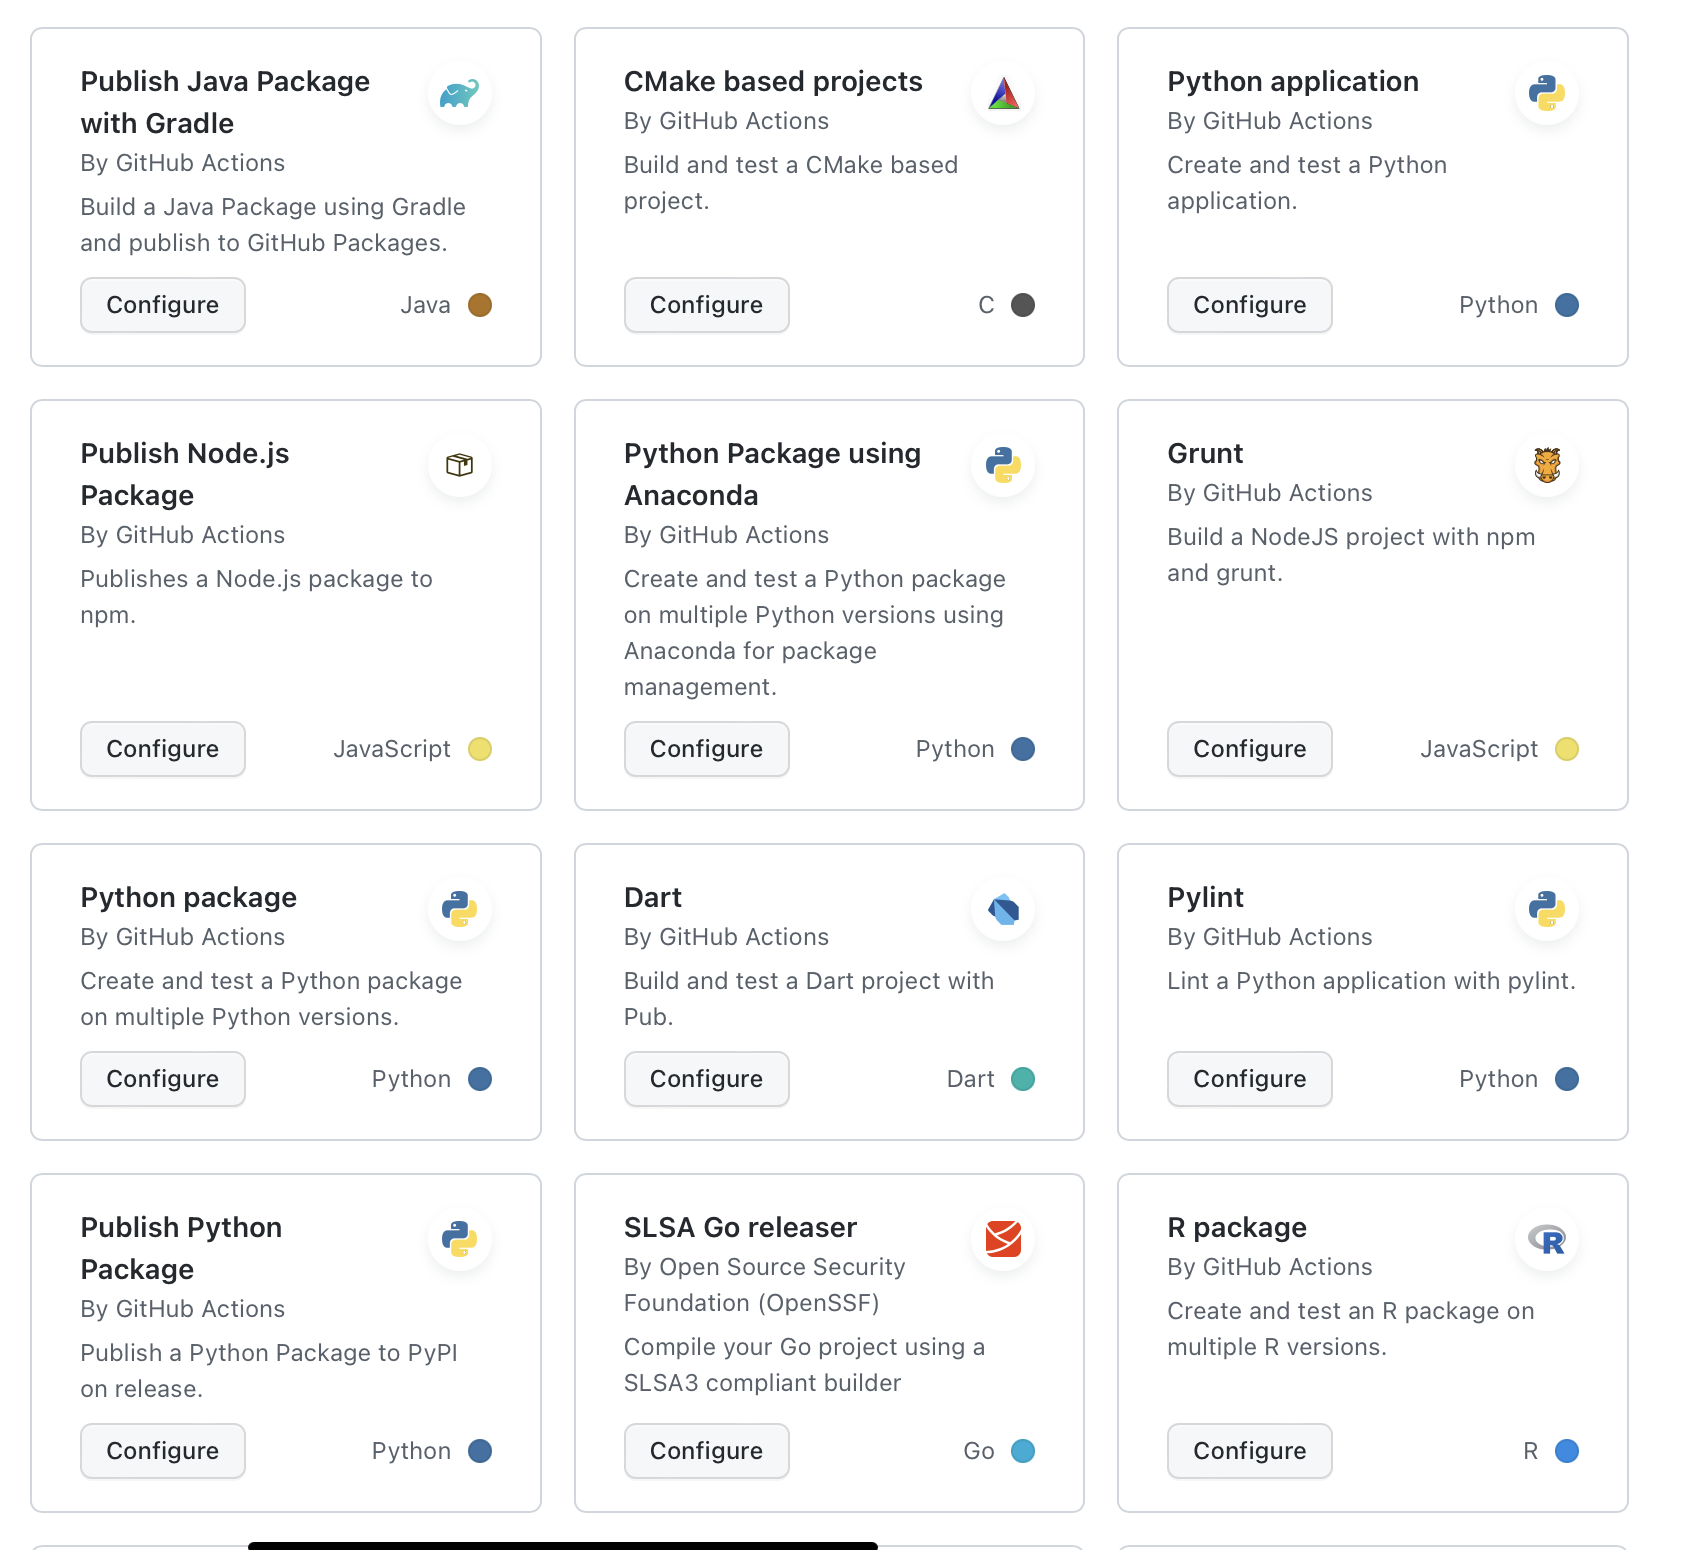
\includegraphics[scale = 0.2]{attachment/chapter_2/Scc103}
	\caption{Github Action/Python}
\end{figure}

Im weiteren werden drei Fälle für das Testen von Python Packete beschrieben.
\begin{itemize}
	\item Python Package using only pip
	\item Python Package using Anaconda
	\item Python Package using Anaconda using tox also locally
	\item Python Applikation using Anaconda
\end{itemize}

\paragraph{Python Package using only pip}
Diese vorkonfigurierte GitHub Aktion installiert alle Dependenies über pip und führt flake8 und pytest aus. Bei Flake8 sind weiter Bedingungen angegeben.

\begin{lstlisting}[style=Config, caption={GitHub Action Temple: Python Package create and test with conda}, captionpos=b]
	
	# This workflow will install Python dependencies, run tests and lint with a variety of Python versions
	# For more information see: https://docs.github.com/en/actions/automating-builds-and-tests/building-and-testing-python
	
	name: Python package
	
	on:
	push:
	branches: [ "main" ] // checks if commit is to main 
	pull_request:
	branches: [ "main" ] // checks if merge request is to main
	
	jobs:
	build: // job_id
	
	runs-on: ubuntu-latest 
	// Linus OS;
	// Caution Linux commands; 
	// one os system (no matrix strategy)
	strategy:
	fail-fast: false // unclear
	matrix:
	python-version: ["3.8", "3.9", "3.10"] // test three python versions
	
	steps:
	- uses: actions/checkout@v3 // find commit (incl. merge) point; checkout version 3
	- name: Set up Python ${{ matrix.python-version }} 
	uses: actions/setup-python@v3 // setup action version 3
	with: // given parameters
	python-version: ${{ matrix.python-version }} // setup specific version
	- name: Install dependencies
	run: | // multiple commands
	python -m pip install --upgrade pip // update pip
	python -m pip install flake8 pytest // install test package
	if [ -f requirements.txt ]; then pip install -r requirements.txt; fi
	// -f requirements.txt checks, if the file has a url (if lokal; file://)
	// if the url is found, the dependencies can be installed.
	// linux shell if [<condition>] then; <Statmant>; fi with no else part
	- name: Lint with flake8
	// caution: the setup os is linux
	run: |
	# stop the build if there are Python syntax errors or undefined names
	flake8 . --count --select=E9,F63,F7,F82 --show-source --statistics
	# exit-zero treats all errors as warnings. The GitHub editor is 127 chars wide
	flake8 . --count --exit-zero --max-complexity=10 --max-line-length=127 --statistics
	- name: Test with pytest
	run: |
	pytest
	
\end{lstlisting}
\footnote{
	\href{https://pip.pypa.io/en/stable/cli/pip_install/}{Pip Installations Optionen},
	\href{https://www.tutorialspoint.com/unix/if-fi-statement.htm}{Linus Shell Command} 
}


%%\paragraph{Python Package Anaconda} 

Diese vorkonfigurierte GitHub Action hat den Zweck, die Automatisierung von Tests mit Hilfe von Anaconda durchzuführen.

\begin{lstlisting}[style=Config, caption={GitHub Action Temple: Python Package create and test with conda}, captionpos=b]
	name: Python Package using Conda
	
	on: [push]
	
	jobs:
	build-linux:
	runs-on: ubuntu-latest
	strategy:
	max-parallel: 5
	// general: maximum number of jobs can run paraell
	// unclear, why this setup is requirerd, if matrix strategy is given.
	
	steps:
	- uses: actions/checkout@v3
	- name: Set up Python 3.10
	uses: actions/setup-python@v3
	with:
	python-version: 3.10
	- name: Add conda to system path
	run: |
	# $CONDA is an environment variable pointing to the root of the miniconda directory
	echo $CONDA/bin >> $GITHUB_PATH
	- name: Install dependencies
	run: |
	conda env update --file environment.yml --name base
	// Update existing env 
	// --prune is general needed.
	// --name base it update a env without activating it
	- name: Lint with flake8
	run: |
	conda install flake8
	# stop the build if there are Python syntax errors or undefined names
	flake8 . --count --select=E9,F63,F7,F82 --show-source --statistics
	# exit-zero treats all errors as warnings. The GitHub editor is 127 chars wide
	flake8 . —count —exit-zero —max-complexity=10 —max-line-length=127 —statistics
	- name: Test with pytest
	run: |
	conda install pytest
	pytest
\end{lstlisting}
%TODO: Test
% Conda install configuration 
(Annahme) Damit conda über den Runner ausgeführt werden kann,  ist conda automatisch mit der \textit{base} Umgebung installiert. Die hier vorgegeben \textit{GitHub Action} verwendet diese gleich. Dabei wird mit dem Befehl 
\begin{lstlisting}[style=CMD, caption={github default install dependencies}, captionpos=b]
	conda env update --file environment.yml
\end{lstlisting}\footnote{
	Refernz in LaTex Code %\href{https://docs.conda.io/projects/conda/en/latest/user-guide/tasks/manage-environments.html?highlight=prune#updating-an-environment}{Doc Conda Update Enviroment}
}
ein Update der aktivierte \gls{VEN} durchgeführt. Damit nicht erst eine aktiviert werden muss, wird 

\begin{lstlisting}[style=CMD, caption={conda update option}, captionpos=b]
	... --name base
\end{lstlisting}
verwendet. Dies bedeutet auch, dass keine neue \gls{VEN} installiert werden muss. Dieser Befehl ignoriert auch in der \textit{name:<>} in \textit{requirments}$\_$\textit{conda.yml}.\\

Für den lokale Nutzung wird die Option

\begin{lstlisting}[style=CMD, caption={conda prune option}, captionpos=b]
	... --prune
\end{lstlisting}
verwendet. Diese deinstalliert alle Abhängigkeiten, welche nicht mehr benötigt werden:

\begin{lstlisting}[style=CMD, caption={Gesamthafter Befehl für lokalen Gebrauch}, captionpos=b]
	conda env update --file requirements_conda.yml --prune
\end{lstlisting}

\paragraph{Python Application}
Für das Testen von Applikationen werden fast identische Workflows benötigt, als für das Testen von Packages.
\begin{lstlisting}[style=Config, caption={GitHub Action Temple: Python Package create and test with conda}, captionpos=b]
	
	# This workflow will install Python dependencies, run tests and lint with a single version of Python
	# For more information see: https://docs.github.com/en/actions/automating-builds-and-tests/building-and-testing-python
	
	name: Python application
	
	on:
	push:
	branches: [ “main” ]
	pull_request:
	branches: [ “main” ]
	
	permissions:
	contents: read
	# The workflow Github token can be granted different permissions.
	
	jobs:
	build:
	
	runs-on: ubuntu-latest
	
	steps:
	- uses: actions/checkout@v3
	- name: Set up Python 3.10
	uses: actions/setup-python@v3
	with:
	python-version: “3.10”
	- name: Install dependencies
	run: |
	python -m pip install —upgrade pip
	pip install flake8 pytest
	if [ -f requirements.txt ]; then pip install -r requirements.txt; fi
	- name: Lint with flake8
	run: |
	# stop the build if there are Python syntax errors or undefined names
	flake8 . —count —select=E9,F63,F7,F82 —show-source —statistics
	# exit-zero treats all errors as warnings. The GitHub editor is 127 chars wide
	flake8 . —count —exit-zero —max-complexity=10 —max-line-length=127 —statistics
	- name: Test with pytest
	run: |
	pytest
\end{lstlisting}

In dem Fall wird die Berechtigung \textit{contents} auf Leserechte gesetzt. Permissions verhindern ungewollte Aktionen von Worksflows.

\paragraph{Python Package - tox local and in cloud}
Um Tox lokal und über GitHub Action ausführen zu können wird \textit{tox-gh-actions} benötigt. Um die Steuerung zu regeln. Die weiteren Test-Packete werden darüber geregelt.

\begin{lstlisting}[style=Config, caption={Own GitHub Action config}, captionpos=b]
	name: Python Package using Conda
	
	on: [push]
	
	jobs:
	build-linux:
	runs-on: ${{matrix.os}}
	strategy:
	os: [ubuntu-latest, windows-latest]
	python-version: ["3.8", "3.9", "3.10"]
	
	steps:
	- uses: actions/checkout@v3
	- name: Set up Python 3.10
	uses: actions/setup-python@v3
	with:
	python-version: ${{matrix.python-version}}
	- name: Add conda to system path
	run: |
	# $CONDA is an environment variable pointing to the root of the miniconda directory
	echo $CONDA/bin >> $GITHUB_PATH
	- name: Install dev dependencies
	run: |
	conda env update --file environment.yml --name base    
	- name: Test with cloud tox
	run: pip install tox tox-gh-actions
	#test, if conda install tox tox-gh-action works
	- name: Test with tox
	run: tox
\end{lstlisting}
Für das lokale ausführen von tox wird \underline{tox-gh-actions} nicht benötigt. Dies regelt die unterschiedliche Behandlung. In der \textit{tox.ini} wird die Konfiguration dafür neu angelegt.

\begin{lstlisting}[style=Config, caption={Update tox.ini with gh-action}, captionpos=b]
	# ============================================================================
	# TOX CONFIGURATION: behave
	# ============================================================================
	# REQUIRES: pip install tox
	# Local and GitHub Action Option
	
	[tox]
	miniversion = 3.8.0							# required minimal tox version
	envlist = py36, py37, py38, flake8, mypy # to check python version
	
	[gh-actions]									# GitHub Action Runner config
	python = 
	3.6 = py36, flake8, mypy
	3.7 = py37
	3.8 = py38
	3.9 = py39
	
	[testenv] 									# Standard python enviroments
	deps=	-r{toxinidir}/requirements_dev.txt # delivers the dependencies
	commands = pytest --basetemp={envtmpdir} {postargs:varialbe} # clear temp directory
	setenv = 
	PYTHONPATH = {toxinidir}				# currently unclear, why it is used
	
	[testenv:flake8]
	basepython = python3.6
	deps = flake8
	commands = flake 8 scr tests
	
	[testenv:mypy]
	basepython = python3.6
	deps=	-r{toxinidir}/requirements_dev.txt # delivers the dependencies
	commands = mypy scr
	
\end{lstlisting}

%TODO: Test
% test if this works if conda installs the both packages

\subsubsection{Secrets and Permissions}
\paragraph{Assigning permission to jobs}  Die Option, \textit{permissions}, konfiguriert die Rechte für den Workflow. 

\begin{lstlisting}[style=Config, caption={Example Permission}, captionpos=b]
	...
	permissions:
	contents: read
	# The workflow Github token can be granted different permissions.
	...
\end{lstlisting}

Jedes Github Action $\leftrightarrow$ Workflow bekommt einen \textit{GITHUB}$\_$TOKEN. Dies wird genutzt, um den Workflow zu authentifizieren. Durch die Einstellungen können ungewollte Effekte von dem Workflow verhindert werden.
\footnote{
	\href{https://docs.github.com/en/actions/using-jobs/assigning-permissions-to-jobs}{Doc Github Permission for Job}
}

\paragraph{Secrets}
GitHub bietet Zugangsdaten unter \textit{Secrets} zu hinterlegen.

\begin{figure}[H]
	\centering
	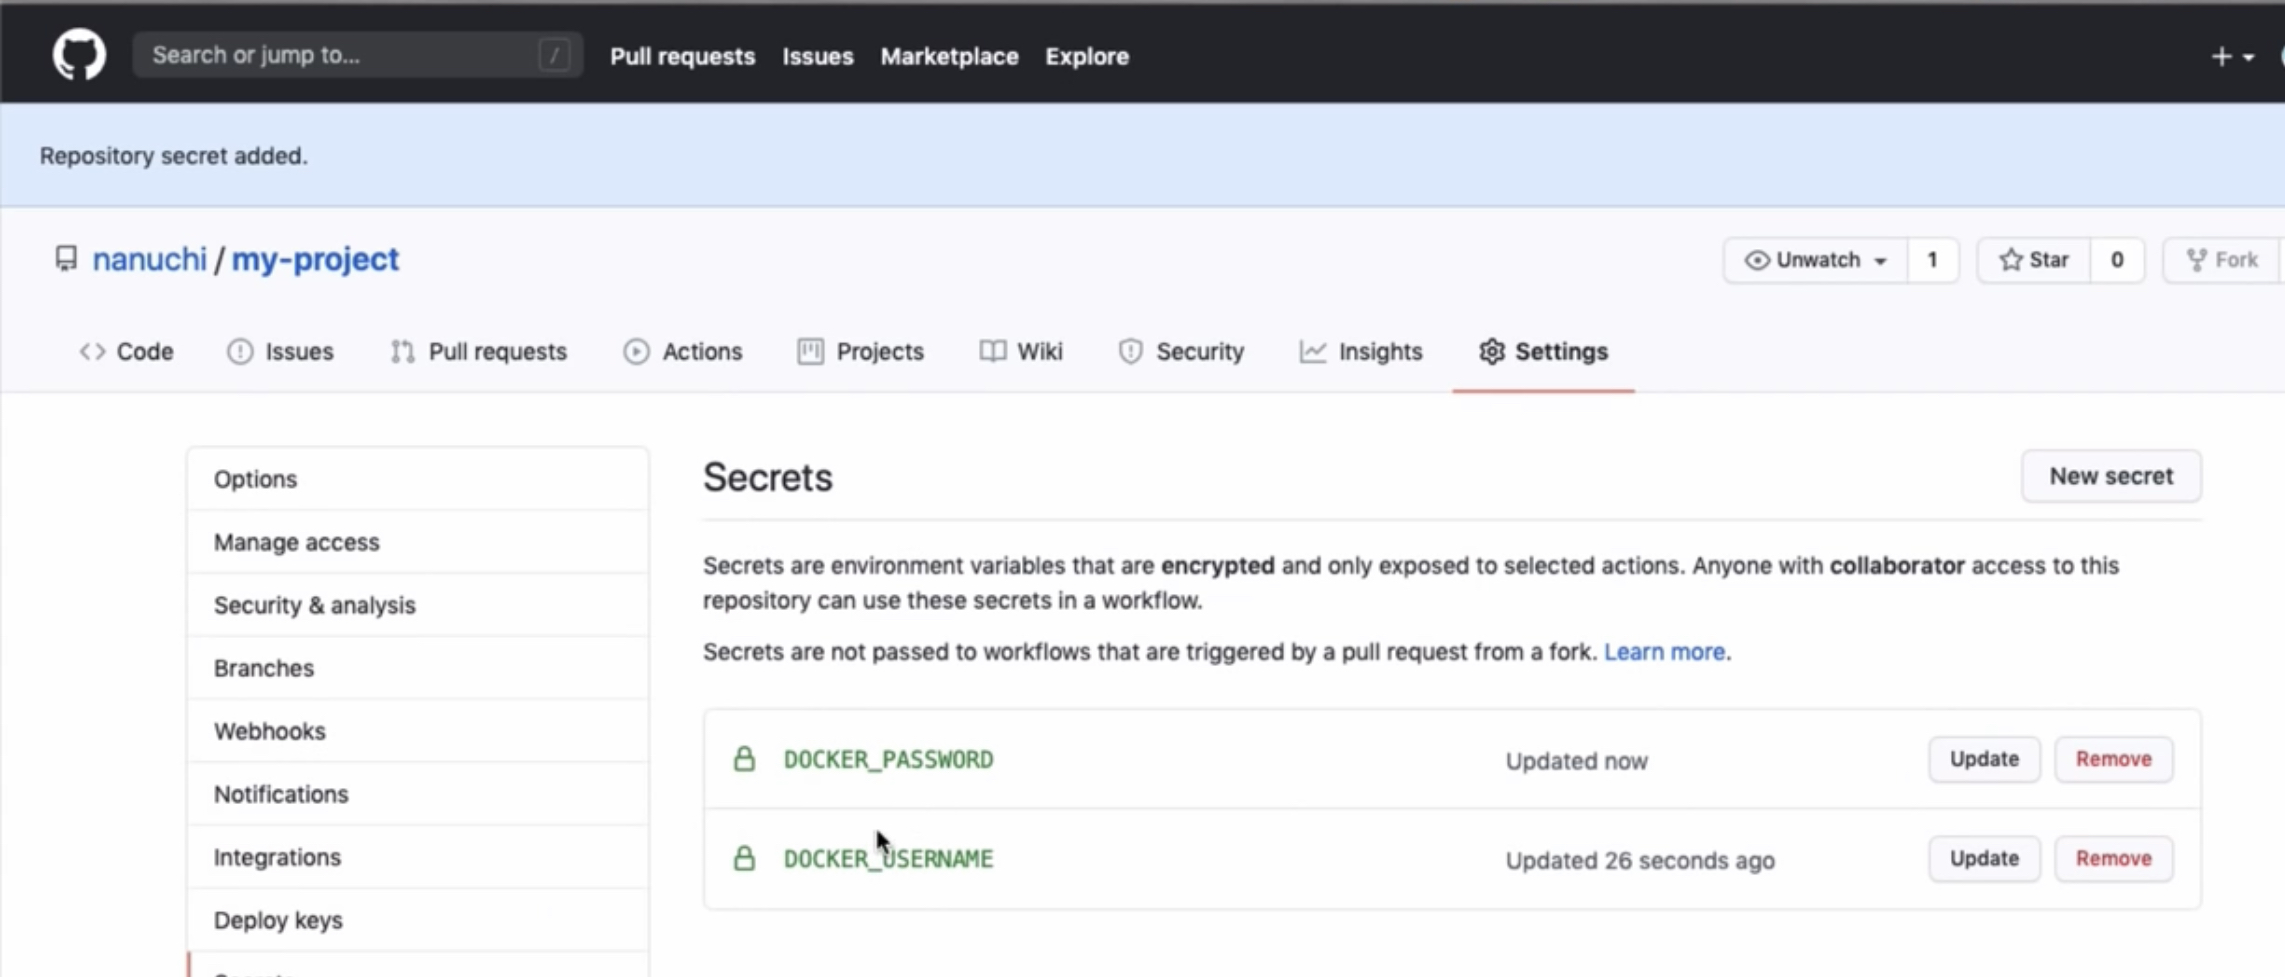
\includegraphics[scale = 0.2]{attachment/chapter_2/Scc105}
	\caption{Github Action/Python}
\end{figure}
Dabei wird ein Verschlüsslung oder Code hinterlegt.

\begin{figure}[H]
	\centering
	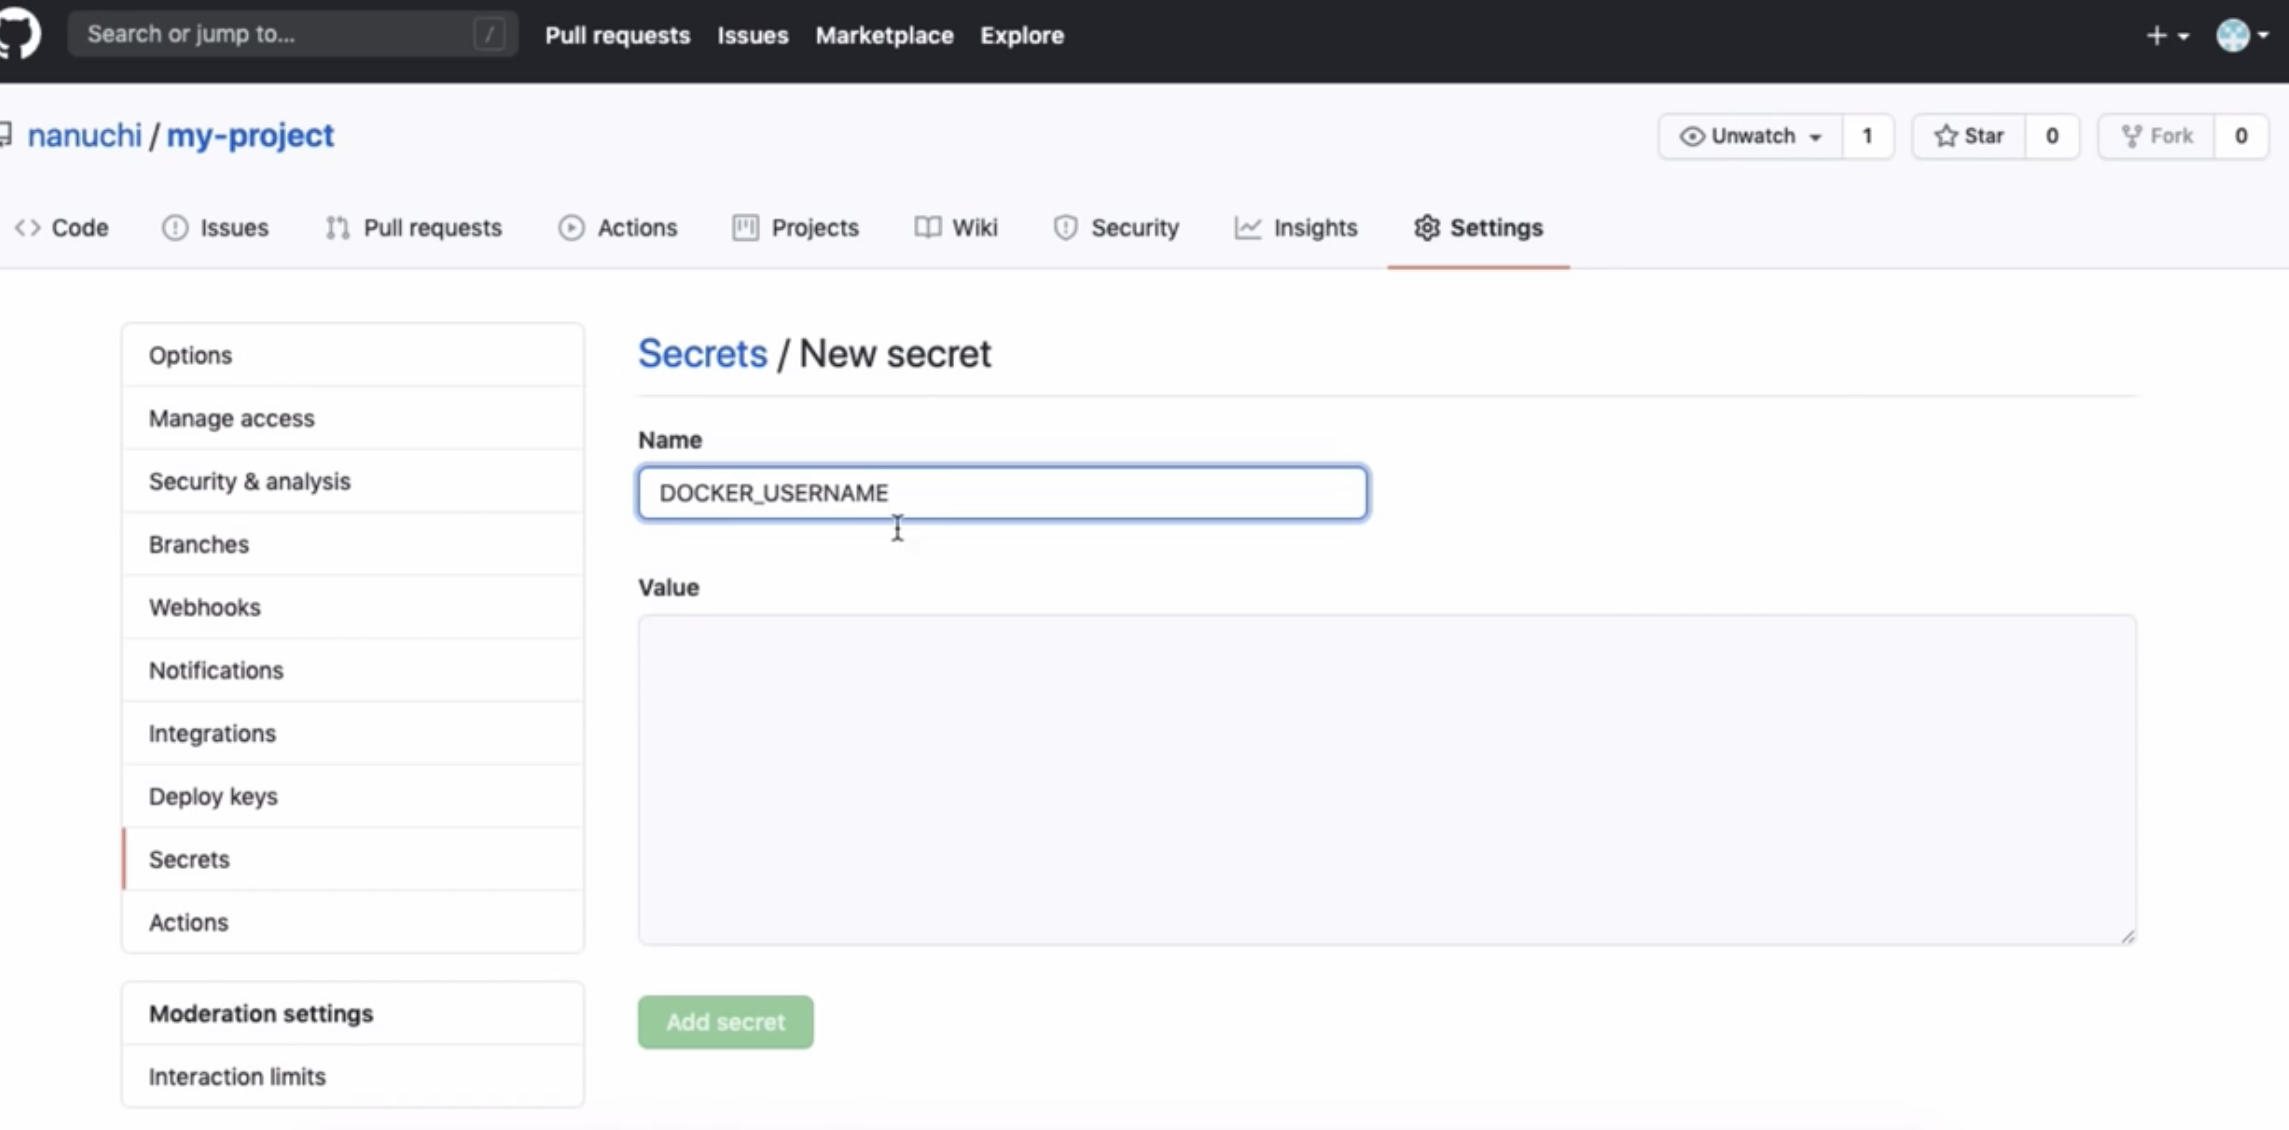
\includegraphics[scale = 0.2]{attachment/chapter_2/Scc106}
	\caption{Github Action/Python}
\end{figure}

Über $\$ \left\lbrace \left\lbrace secrets.<Secret Name> \right\rbrace\right\rbrace$ wird diese angelegt.

\begin{lstlisting}[style=Config, caption={Example Secrets}, captionpos=b]
	...
	name: Build docker image
	uses: mr-smithers-excellent/docker-build-push@4
	with:
	image: nanajanashia/demo-app
	regestriy: dock.io
	username:${{secrets.DOCKER_USERNAME}}
	password:${{secrets.DOCKER_PASSWORD}} 
	...
\end{lstlisting}
